\documentclass[11pt]{article}

%\usepackage[utf8]{inputenc}
\usepackage{indentfirst}
\usepackage{float}
\usepackage{array}
\usepackage{listings}
\usepackage{csquotes}
\usepackage{enumitem, amsmath, amssymb, amsfonts, latexsym, mathrsfs}
\usepackage{graphicx}
\usepackage{subfig}
%\usepackage[greek,english]{babel}
%\usepackage{alphabeta}
\usepackage{multicol}
\usepackage{bookmark}

\usepackage{caption}
\captionsetup[figure]{font={small,it},labelfont={bf},justification={raggedright},singlelinecheck={false},name={Figura.}}

\usepackage{blindtext}

\usepackage{biblatex}
\addbibresource{bibliography.bib}

\usepackage[a4paper, total={6in, 8in}]{geometry}

% Tipografía
\usepackage{helvet}
\renewcommand{\familydefault}{\sfdefault}
\usepackage[sfdefault]{carlito}
\usepackage{comment}

% Imagenes
\graphicspath{ {./Images/} }

% Interlineado
\usepackage{setspace}
\spacing{1.15}

% Setup de hiperenlaces
%\usepackage[hidelinks]{hyperref}
\hypersetup{
    colorlinks=true,
    linkcolor=cyan,
    filecolor=magenta,      
    urlcolor=cyan,
    pdftitle={Jiménez Montero Jesús Crying Girl in the Border}
	citecolor=cyan
}

% Número de página
\usepackage{fancyhdr}
\pagestyle{fancy}
\rhead[]{}
\lhead[]{}
\renewcommand{\headrulewidth}{0pt}
\rfoot[]{}
\lfoot[LF-even] {\hrulefill \newline \raggedright{\hyperref[fig:foto]{\textit{Volver a fotografía}}} --- \raggedleft{\Large{\textbf{\thepage}}}}
\cfoot[]{}



%______________________________________________________________________________
%______________________________________________________________________________
%______________________________________________________________________________
%______________________________________________________________________________
\begin{document}

% PORTADA
\begin{titlepage}

	\centering
	\hrule
	\vspace{1cm}
	{\bfseries\Huge Ensayo --- Análisis de fotografía \par}
	\vspace{0.5cm}
	\large{\textbf{Jesús Jiménez Montero} \par}

	\vspace{1cm}

	\begin{figure}[H]

		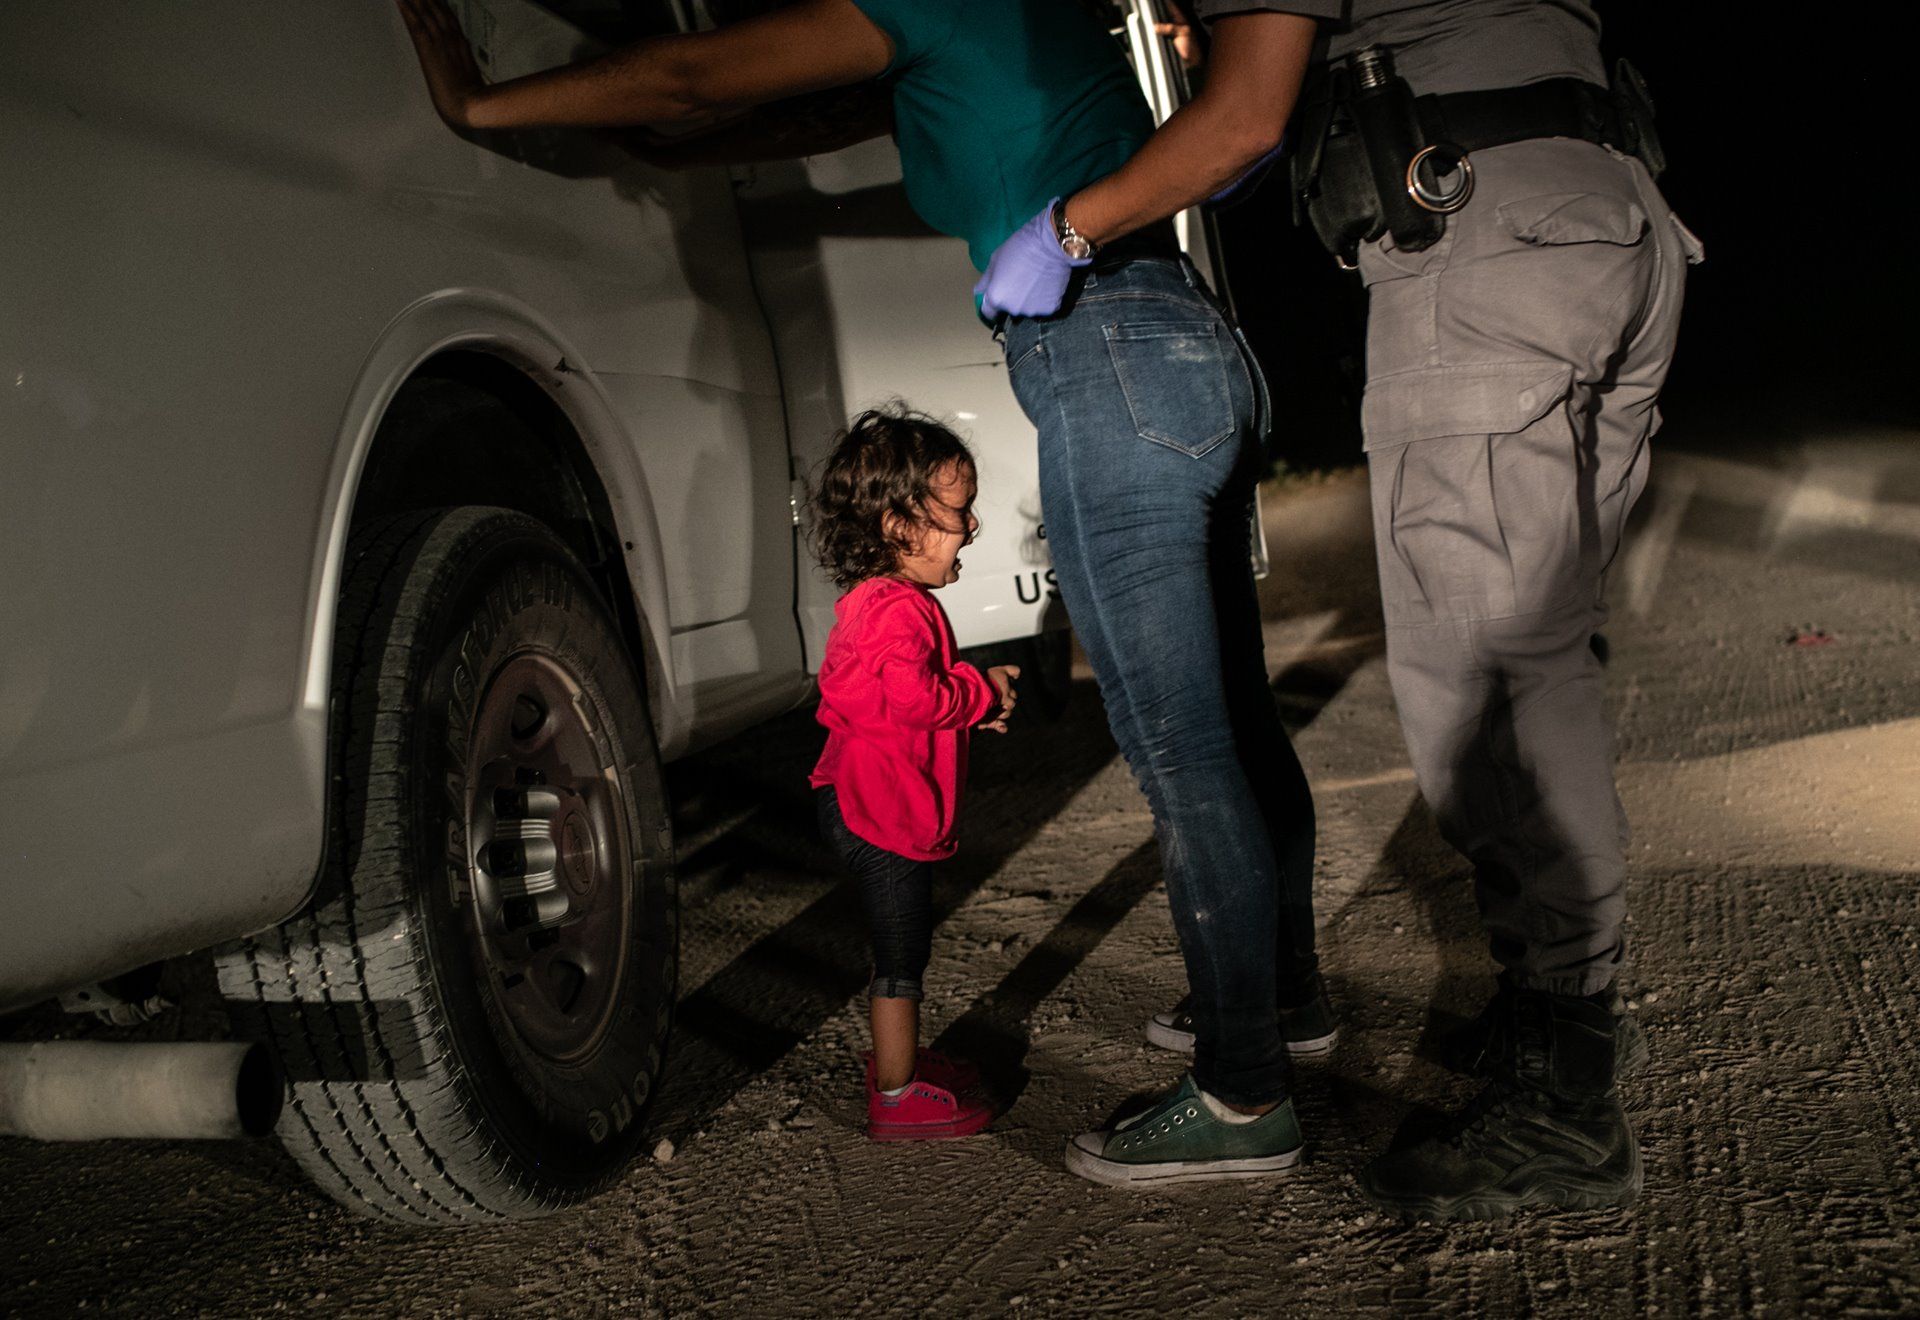
\includegraphics[width=\textwidth,height=\textheight,keepaspectratio]{Images/WPPF-2019PhotoContest-POYNominee-JohnMoore.jpg}
		\caption{{Crying Girl in the Border, John Moore, 18 junio 2018}}\cite{moore-2018}
		\label{fig:foto}

	\end{figure}

	\vspace{0.5cm}

	\vspace{1cm}
	\hrulefill
\end{titlepage}
\newpage

\section{NIVEL CONTEXTUAL}
% NIVEL CONTEXTUAL ____________________________________________________________

En muchas ocasiones demostrar la realidad implica revelar lo que oculta la sociedad detrás de una fachada de irrealidad. \newline

Esto es lo que quiere mostrar el fotógrafo americano John Moore con esta fotografía realizada en junio de 2018, coincidiendo con la nueva política de Trump relacionada con “cero tolerancia” los inmigrantes, siendo procesados como criminales. Mayoritariamente, esto significaba que los niños eran separados de sus padres, siendo la niña de la foto, Yanela Sánchez, también separada de su madre, Sandra Sánchez, siendo llevada a custodia. \newline

Podemos definir esta fotografía en el género fotográfico de “prensa” siendo el género más prominente en la fotografía debido a que John Moore es un periodista y fotógrafo para Getty Images \cite{world-press}. También podemos encontrar otros géneros algo más ocultos, ya que en la fotografía contiene un componente social muy marcado, llamando y criticando como se gestionan los inmigrantes en Estados Unidos de formas inhumanas e irrespetuosas. De hecho, la indignación que sucedió a la publicación de la fotografía, ocasionó que se revirtiese esta política de “cero tolerancia” el 20 de junio de 2018. \cite{hanna-2019} \newline

Aun así, no todo el mundo recibió esta fotografía de la misma manera. Posteriormente a la publicación de la fotografía, otros medios declararon que las familias nunca fueron separadas. Esta información procedió del padre (Danis Javier Varela Hernández) \cite{sacks-2018}, el ministro de Asuntos Exteriores de Honduras (Nelly Jerez) \cite{palencia-2019} y Aduanas y Protección de Fronteras de Estados Unidos \cite{sacks-2018}. \newline

Hablando un poco del fotógrafo de esta imagen, se trata de John Moore, un fotógrafo estadounidense que ha trabajado para Getty Images desde 2007. John Moore citó esto cuando hizo la fotografía: \textit{Traducido del inglés por mí: "Como un fotoperiodista, mi trabajo consiste en informar y reportar sobre lo que está ocurriendo, aunque, creo que también es importante humanizar los problemas que normalmente se omiten en las estadísticas."} \cite{moore-2018}; incluso en algunos medios de comunicación declaró que tuvo que "parar y respirar" \cite{moore-2018} después de tomar la fotografía. \newline

Hablando sobre aspectos más técnicos de la imagen, \textit{World Press Photo} \cite{moore-2018} nos provee con las características técnicas de la imagen. La fotografía se disparó en la frontera de Estados Unidos, más concretamente, en la frontera de McAllen, Texas \cite{einstein}. La cámara usada fue Canon EOS-1D X Mark II \cite{canon}. Una parte muy importante de la fotografía es la sensación de cercanía que otorga la imagen. Se consiguió con objetivo con longitud focal de 35 mm. \newline


\section{NIVEL MORFOLÓGICO}
% NIVEL MORFOLÓGICO ___________________________________________________________
La imagen contiene una gran cantidad de puntualidades que elaboran una composición bastante cargada, en el que podemos destacar cuatro puntos. Enumerándolos de izquierda a derecha:
\begin{enumerate}
	\item El vehículo.
	\item La niña, más concretamente, su sudadera.
	\item Los pantalones de la madre (y por extensión, la madre.)
	\item Los pantalones del guardia (mismo caso que antes, por extensión, el guardia.)
\end{enumerate}

\begin{figure}[H]
	
\includegraphics[scale = 0.3]{Images/dot.png}
	\caption{Puntos de interés en la imagen.}
\end{figure}

La fotografía se compone de manera que se incluye a todos los sujetos en el mismo plano. Además, la amplitud del encuadre demuestra ser un plano general en el que no se puede discernir otros elementos fuera de campo. Asimismo, la fotografía contiene, de forma menos prominente, líneas. Es decir, las líneas que se sitúan en el terreno y la camioneta guían al espectador a lo que está ocurriendo en la fotografía. \newline 

Siendo una fotografía nocturna y probablemente realizada a prisa y corriendo por el fotógrafo, da como resultado una imagen con cierta pérdida de nitidez que podemos achacar a la falta de luz y que la imagen se realizara con valores de ISO relativamente altos. Introduciendo ruido digital en la fotografía y raíz de esto, una pérdida de nitidez. \newline

Aunque, la pérdida de la nitidez y la introducción de cierta borrosidad gana en favor de la imagen, creando una sensación de urgencia y confusión que se refleja en la imagen. Probablemente, la persona que vea esta imagen le entre le otorgue las características anteriormente mencionadas.  \newline

Como he explicado antes, el hecho de que sea una fotografía nocturna añade el componente de la oscuridad, que en este caso, es un elemento que juega un papel importante en la composición. No obstante, se puede apreciar lo que parece unos faros de un vehículo (\textit{probablemente luces de carretera}), este detalle significa que es posible que haya otras personas fuera de campo que no podemos ver. \newline

En términos más técnicos, la iluminación es artificial con un balance entre dura y suave. El hecho de que al ser de noche y que las luces provengan de un ángulo de 90.º, se produce un balance entre las claves altas (\textit{el hecho de haya una luz muy fuerte}) y la clave baja (\textit{la misma luz crea muchas sombras que se aprecian en el fondo de la composición}). \newline

Otro elemento muy fuerte en esta imagen es el brutal contraste que existe, no entre las luces u otros elementos; sino en la ropa que llevan las personas de la fotografía. La niña destaca prácticamente sobre todo lo demás que rodea a la fotografía, con su ropa roja; además de estar justo delante de una camioneta blanca, añadiendo todavía más contraste a la niña haciéndola destacar todavía más. Esto también ocurre con la madre, pero a un nivel menos elevado, sus pantalones también resaltan al estar delante de la puerta blanca de la camioneta. \newline

\section{NIVEL COMPOSITIVO}
% NIVEL COMPOSITIVO ___________________________________________________________
% TODO: Falta añadir algo relacionado con ritmo, tensión y recorrido visual

Cambiando de tema a composición, podemos empezar por una de las características más comunes en fotografía, la ley de tercios.
\begin{figure}[H]
	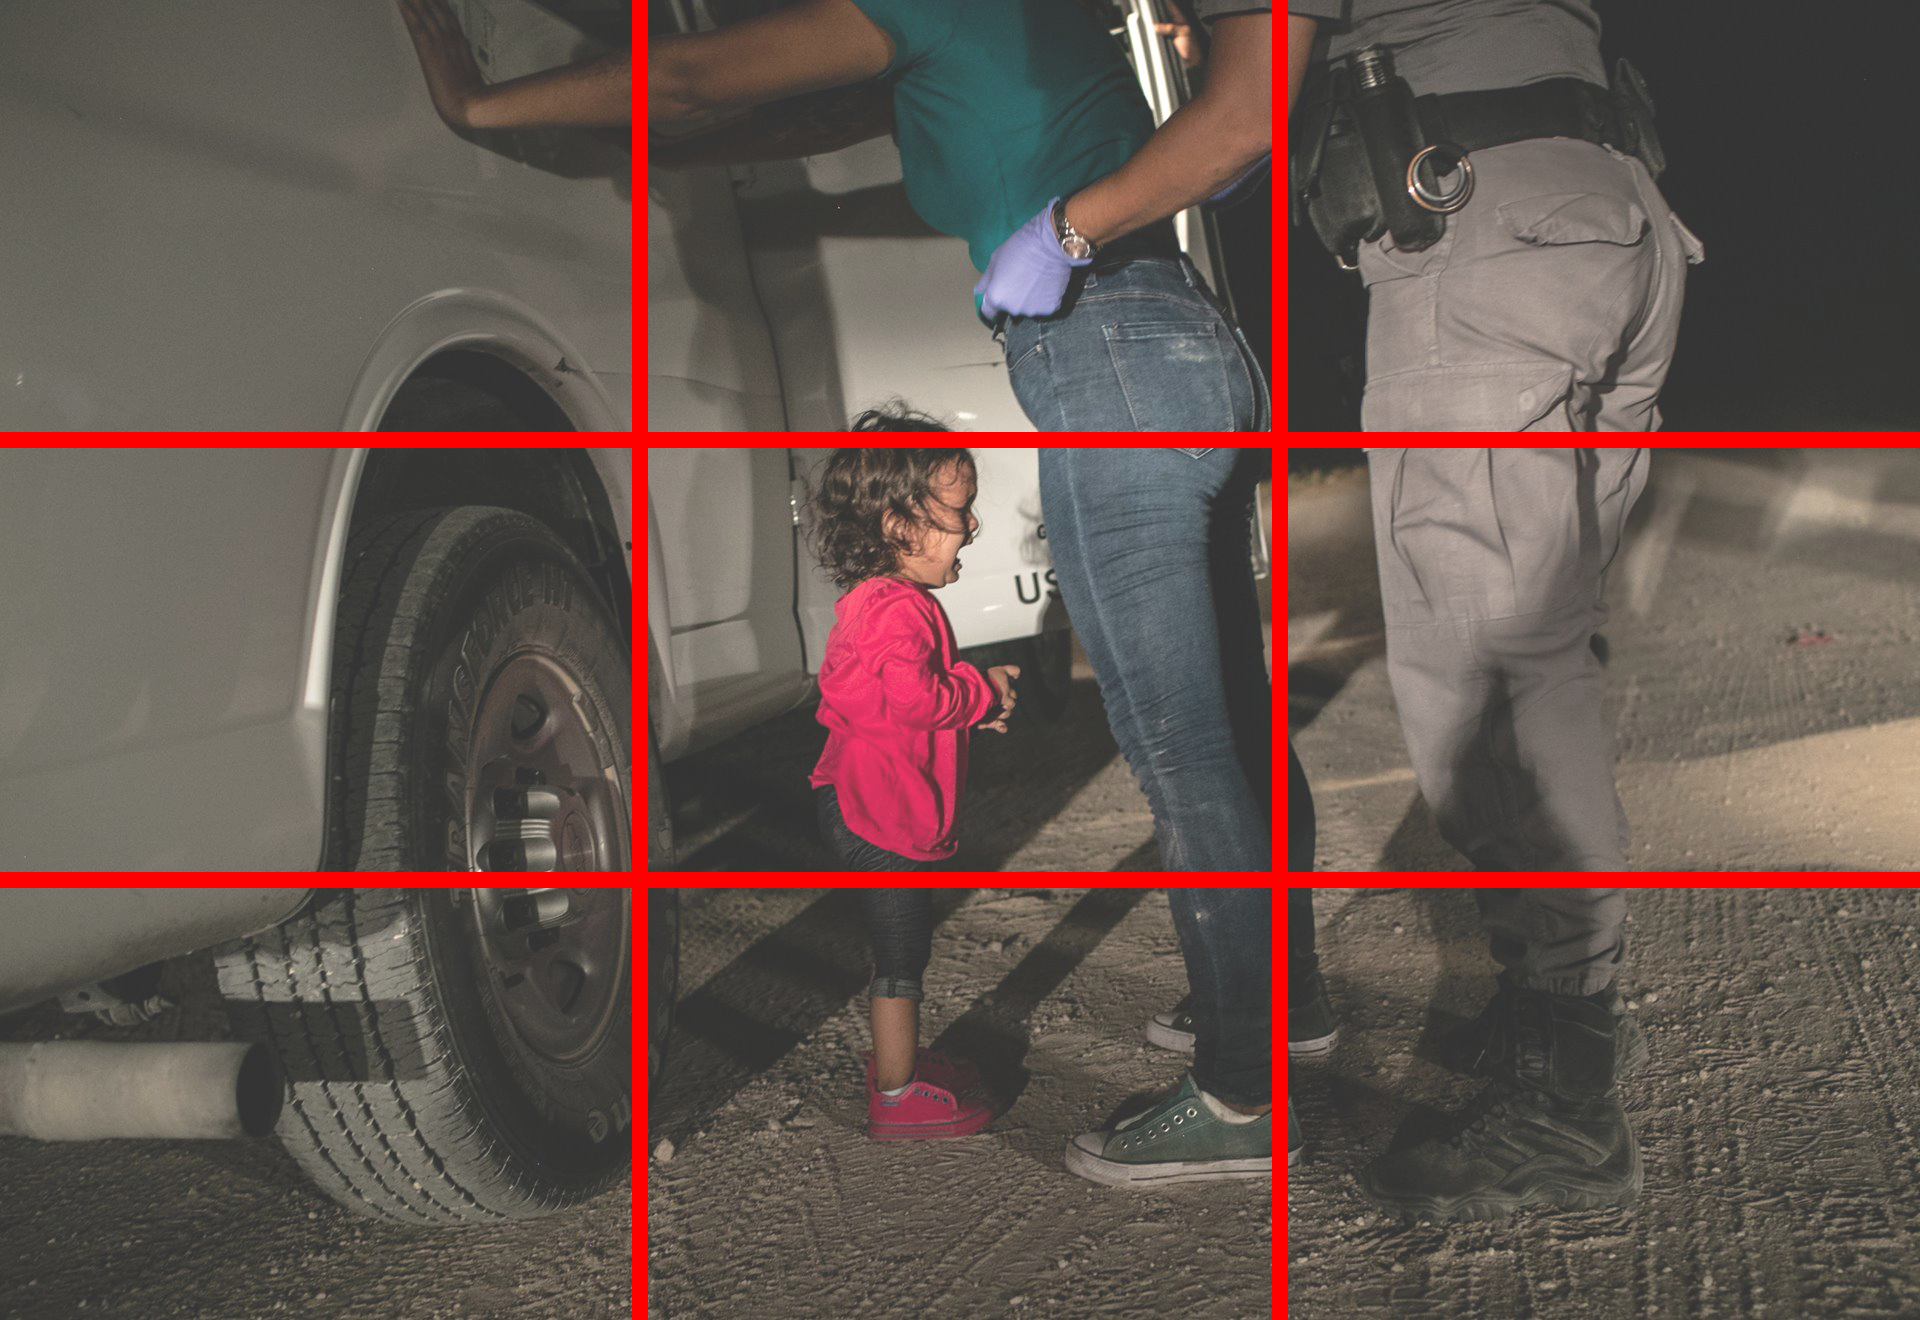
\includegraphics[scale = 0.5]{Images/rulethrids.png}
	\caption{Ley de tercios.}
	\label{fig:rulethrids}
\end{figure}

Podemos observar que la composición es muy variada, situando a la niña en el centro de la imagen, coincidiendo su cabeza y torso con las líneas superior e inferior respectivamente. Mientras que la madre se coloca en el tercio derecho, estando el guardia. Y el coche situado en el tercio izquierdo de la imagen, acaparando todo el tercio. \newline

Se puede destacar de esta imagen su “dentro de campo” o quizás mejor dicho, su falta de “fuera de campo”. En la imagen se puede apreciar el hecho de todo la “acción” ocurre en primer plano y no hay nada más detrás de los sujetos. Se logra con esto una composición bastante cerrada y que no permite sacar la atención de lo que ocurre en primer plano a los espectadores. \newline

Precisamente toda la composición es muy interesante en términos de la instantaneidad del momento que se presenta en esta fotografía. Debido la naturaleza de la fotografía de exponer el momento a más espectadores, la imagen también se representa un momento en el tiempo concreto que lo que ocurrió en el 2019 con la ley de “cero-inmigración” recién implantada por Trump. \newline

\section{NIVEL ENUNCIATIVO}
% NIVEL ENUNCIATIVO ___________________________________________________________

Para terminar el análisis de la fotografía, nos centramos en el nivel enunciativo.
En primer lugar, el punto de vista está claramente situado a la altura de los ojos de la niña, como se puede apreciar en la regla de tercios (\ref{fig:rulethrids}).\newline

El hecho de la cámara esté situada de esta manera añade cierta parte de sensación de pena, ya que nos ponemos al mismo nivel que la niña.
También se incluye el hecho de que la cámara solo permita ver la parte baja de la cintura de los otros dos adultos. La sensación que todo esto crea es la de “falta de poder”, como si la fotografía quisiese decir al espectador: “no tienes poder aquí, tú eres la niña”. \newline

Es más, lo comentado antes se complementa con la actitud que manifiestan los sujetos de la fotografía, el hecho de que solo podemos ver a la niña llorando es una emoción muy fuerte que se complementa con que no podamos ver las expresiones de los otros dos sujetos. Hablando un poco fuera de la imagen, pienso que los espectadores intentan rellenar esas expresiones en su mente. \newline

\newpage

% Bibliografia  _______________________________________________________________
\printbibliography
\newpage

\blinddocument
\end{document}